\section{Experiment 7: Multi-Class Joint Prediction (TTF1 \& CK7)}

\subsection{Rationale and Hypothesis}
Previous experiments treated TTF1 and CK7 status as independent binary classification problems (e.g., TTF1 Positive vs. Negative). However, clinically, these biomarkers often manifest in specific combinations that define distinct lung cancer phenotypes.

Experiment 7 investigates a \textbf{Multi-Class Classification} approach, where a single model predicts one of four mutually exclusive categories representing the combined status of both biomarkers.

\begin{itemize}
    \item \textbf{Hypothesis:} By modeling the joint distribution of TTF1 and CK7, the network may learn shared feature representations that are more robust than training two isolated binary models.
    \item \textbf{Counter-Hypothesis:} Splitting the small dataset into four classes (instead of two) will exacerbate class imbalance and data scarcity, potentially degrading performance below that of individual binary classifiers.
\end{itemize}

\subsection{Methodology}

\subsubsection{Label Definition}
The labels were engineered by combining the binary status of both biomarkers into a single integer target $y \in \{0, 1, 2, 3\}$:
\begin{itemize}
    \item \textbf{Class 0:} TTF1- / CK7-
    \item \textbf{Class 1:} TTF1+ / CK7-
    \item \textbf{Class 2:} TTF1- / CK7+
    \item \textbf{Class 3:} TTF1+ / CK7+
\end{itemize}

\subsubsection{Input Data Processing}
A multimodal approach was selected to maximize information gain:
\begin{enumerate}
    \item \textbf{3D CT Volumes:} Cropped around the lung mask and resized to a target shape of $(128, 128, 128)$. Data augmentation (random flips and rotations) was applied during training.
    \item \textbf{Radiomics:} Handcrafted features were extracted and selected using \texttt{SelectKBest}, reducing the dimensionality to the top 20 discriminative features.
\end{enumerate}

\subsubsection{Model Architecture}
A dual-branch Hybrid Neural Network was constructed:
\begin{itemize}
    \item \textbf{Visual Branch:} A 3D CNN processing the CT volume, consisting of Conv3D blocks, Batch Normalization, and Max Pooling, ending in Global Average Pooling.
    \item \textbf{Tabular Branch:} A Multi-Layer Perceptron (MLP) processing the Radiomics vector.
    \item \textbf{Fusion:} Feature vectors from both branches are concatenated and passed through dense layers with Dropout.
    \item \textbf{Output:} A Dense layer with 4 units using the \texttt{softmax} activation function.
\end{itemize}

\subsection{Experimental Results}

\subsubsection{Deep Learning vs. Machine Learning}
To isolate the effectiveness of the Deep Learning approach, we compared the Hybrid 3D CNN against a gradient boosting model (XGBoost) trained solely on the Radiomics features.

\begin{figure}[htbp]
    \centering
    % INLOCUIESTE 'xgboost_cm.png' CU NUMELE FISIERULUI TAU
    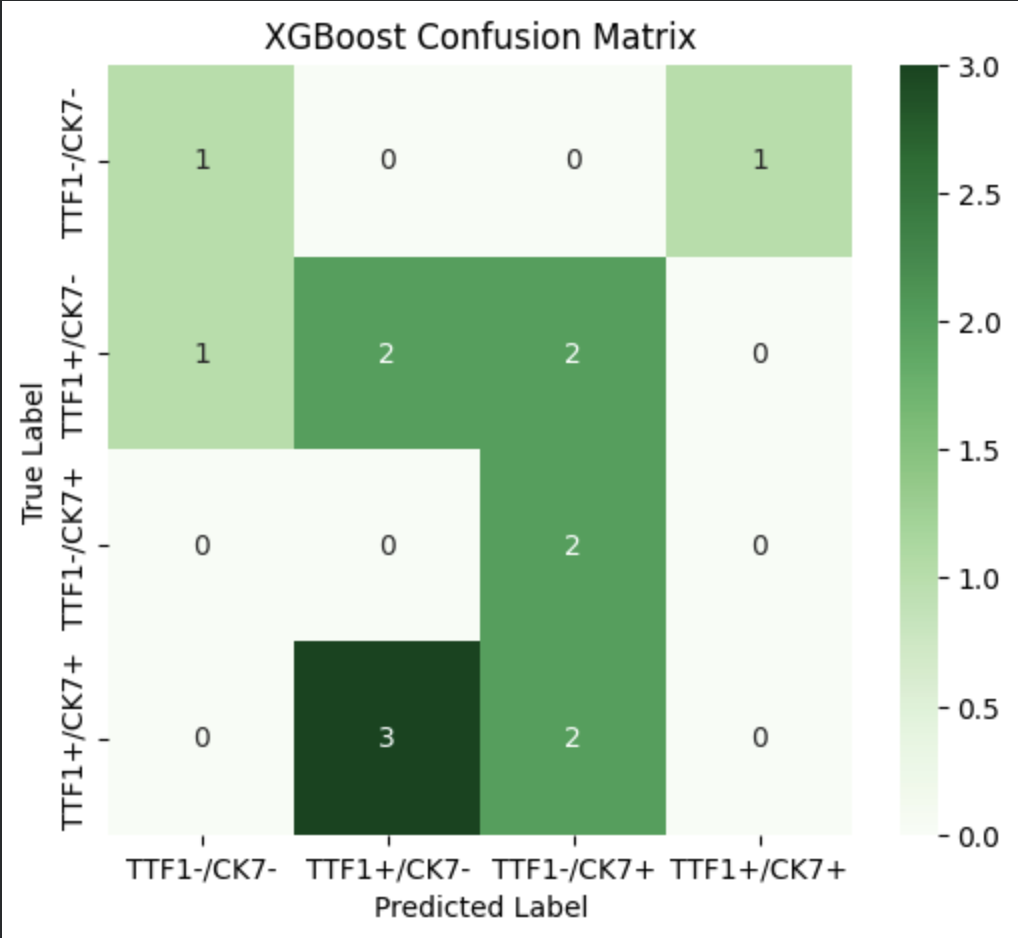
\includegraphics[width=0.6\textwidth]{Screenshot 2025-12-13 at 09.52.28.png} 
    \caption{Confusion Matrix for XGBoost (Radiomics Only).}
    \label{fig:exp7_xgboost}
\end{figure}

\begin{figure}[htbp]
    \centering
    % INLOCUIESTE 'cnn_cm.png' CU NUMELE FISIERULUI TAU
    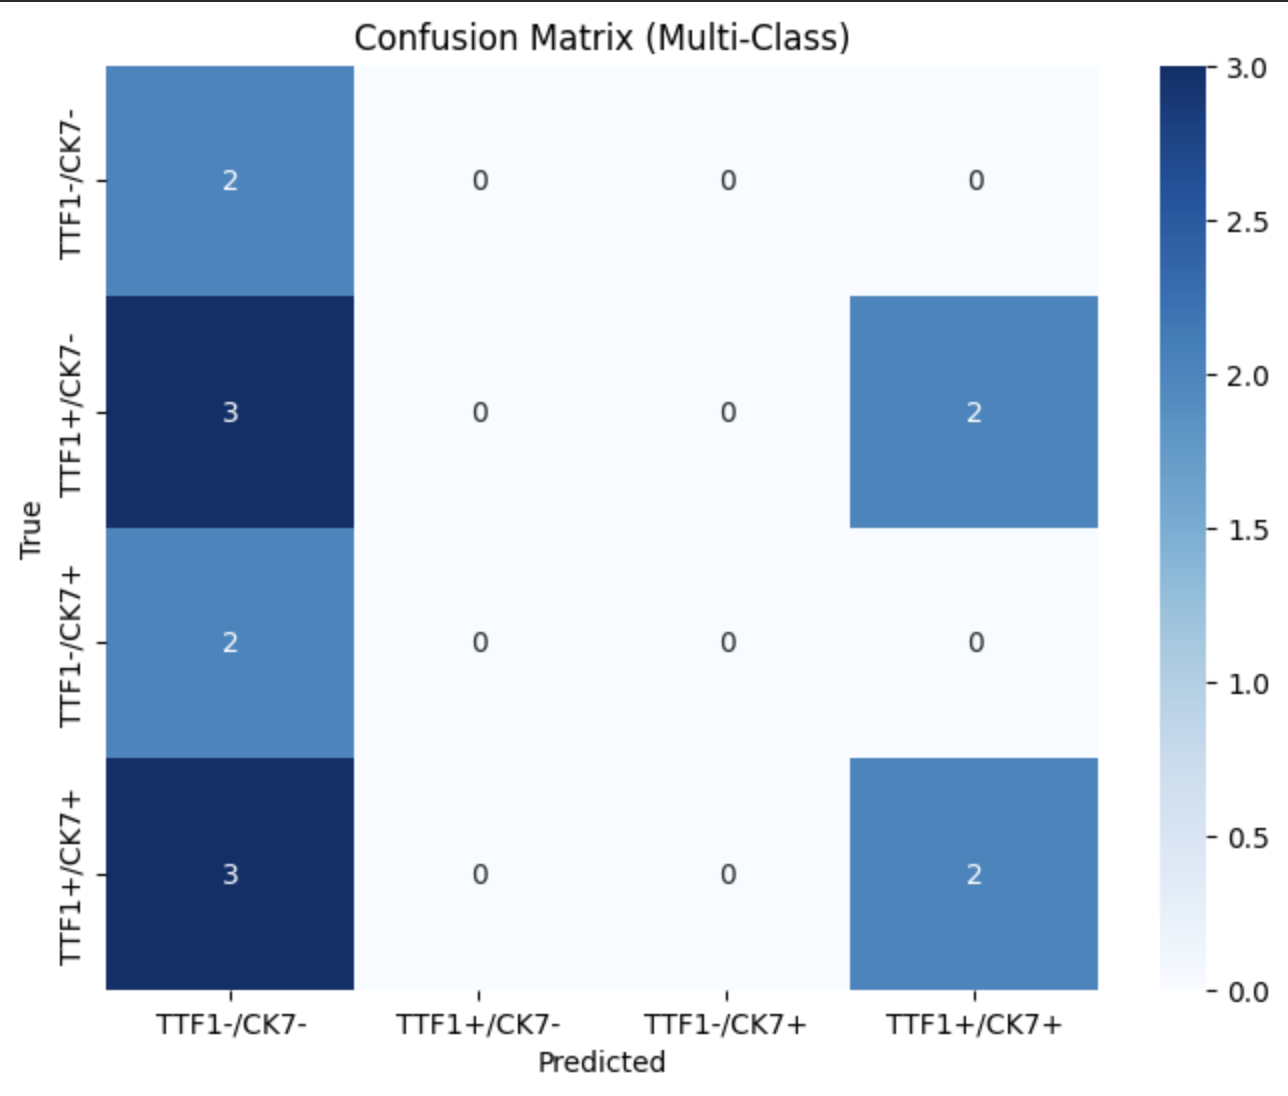
\includegraphics[width=0.6\textwidth]{Screenshot 2025-12-13 at 09.53.46.png}
    \caption{Confusion Matrix for Hybrid 3D CNN.}
    \label{fig:exp7_cnn}
\end{figure}

\subsubsection{Performance Metrics}
The models were evaluated on the stratified test set ($N=14$).

\begin{itemize}
    \item \textbf{3D CNN (CT Only):} The model failed to generalize, achieving an accuracy of only $\approx 14\%$, predicting the majority class or random noise.
    \item \textbf{Hybrid 3D CNN (CT + Radiomics):} Performance remained low ($\approx 21\%$), with the model struggling to differentiate between the four distinct classes.
    \item \textbf{XGBoost (Radiomics Only):} This approach yielded the highest accuracy ($\approx 36\%$). While still low, it demonstrated a better ability to identify Class 3 (TTF1+/CK7+) compared to the deep learning models.
\end{itemize}

\subsection{Conclusion of Experiment 7}
This experiment demonstrates the "Curse of Dimensionality" regarding the output space.
\begin{enumerate}
    \item \textbf{Data Scarcity:} With a total dataset of $\approx 87$ patients split into 4 classes, some classes (e.g., Class 0 and Class 2) had extremely few samples in the training set. The DL model could not learn robust features from such sparse examples.
    \item \textbf{Radiomics Superiority:} Handcrafted features (Radiomics) proved more robust to the small sample size than raw pixel data, as evidenced by XGBoost outperforming the CNN.
    \item \textbf{Recommendation:} For this specific dataset size, independent binary classifiers (Experiment 2-5 approach) are superior to a joint multi-class formulation.
\end{enumerate}